\documentclass[
	tikz,
	convert={outext=.svg, command=\unexpanded{pdf2svg \infile\space\outfile}}
	]{standalone}

\usepackage{tikz}
\usepackage{xfp}

\definecolor{blueviolet}{HTML}{8A2BE2}
\definecolor{brightgreen}{HTML}{44CC11}

\begin{document}
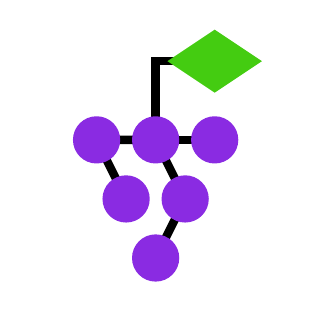
\begin{tikzpicture}

\def\width{3.25}
\def\height{3.25}
\def\offx{0}
\def\offy{0.20}
\def\ox{\fpeval{\width /2+\offx}}
\def\oy{\fpeval{\height /2+\offy}}

%\def\circled{0.25}
%\def\linew{3pt}
%\def\diamondw{0.45}
%\def\diamondh{0.30}

\def\circled{0.30}
\def\linew{3pt}
\def\diamondw{0.60}
\def\diamondh{0.40}

\path [use as bounding box] (0,0) rectangle (\width,\height);

% Lines
\draw [line width=\linew] (\ox,\oy)
	+(-0.375,-0.75)
	-- +(-0.75,0)
	-- +(0,0)
	-- +(0.375,-0.75)
	-- +(0,-1.5);

\draw [line width=\linew] (\ox,\oy)
	-- +(0.75,0);

\draw [line width=\linew] (\ox,\oy)
	-- +(0,1)
	-- +(0.75,1);

% Circles
\fill [fill=blueviolet] (\ox,\oy)
	+(-0.75,0) circle (\circled)
	+(0,0) circle (\circled)
	+(0.75,0) circle (\circled)
	+(-0.375,-0.75) circle (\circled)
	+(0.375,-0.75) circle (\circled)
	+(0,-1.5) circle (\circled);

% Diamond	
\fill [fill=brightgreen] (\ox,\oy) ++(0.75,1)
	+(-\diamondw,0) --
	+(0,-\diamondh) --
	+(\diamondw,0) --
	+(0,\diamondh) --
	cycle;

% Center without bounding box
%\path (\ox,\oy) ++(-0.75,1) +(-\diamondw,0);

\end{tikzpicture}
\end{document}

